\documentclass[conference]{IEEEtran}
%\IEEEoverridecommandlockouts
% The preceding line is only needed to identify funding in the first footnote. If that is unneeded, please comment it out.
\usepackage{cite}
\usepackage{amsmath,amssymb,amsfonts}
\usepackage{algorithmic}
\usepackage{graphicx}
\usepackage{textcomp}
\usepackage{xcolor}

\usepackage{proof}
\usepackage{amsmath,amssymb,amsthm,textcomp}

\usepackage{booktabs}   %% For formal tables:
%% http://ctan.org/pkg/booktabs
\usepackage{wrapfig}
\usepackage{subcaption} %% For complex figures with subfigures/subcaptions
%% http://ctan.org/pkg/subcaption

\usepackage{url}
\usepackage{xspace}
\usepackage{flushend}

\usepackage{fancyvrb}
\fvset{fontsize=\smaller}

\usepackage{color}

\usepackage{hyperref}
\usepackage{cleveref}

\def\BibTeX{{\rm B\kern-.05em{\sc i\kern-.025em b}\kern-.08em
    T\kern-.1667em\lower.7ex\hbox{E}\kern-.125emX}}
%%% Todo comments

%% Comment out one of these two definitions.
% \newcommand{\todo}[1]{\relax}
\newcommand{\todo}[1]{{\color{red}\bfseries [[#1]]}}

% Don't show todo commands if this macro is defined.
\ifdefined\notodocomments
  \renewcommand{\todo}[1]{\relax}
\fi

\newcommand{\ourTypeSystem}{our type system\xspace}
\newcommand{\OurTypeSystem}{Our type system\xspace}
\newcommand{\theDeterminismChecker}{the Determinism Checker\xspace}
\newcommand{\TheDeterminismChecker}{The Determinism Checker\xspace}
\newcommand{\theDeterminismCheckerImplementation}{\theDeterminismChecker implementation\xspace}
\newcommand{\TheDeterminismCheckerImplementation}{\TheDeterminismChecker implementation\xspace}

% A commit hash
% \newcommand{\commit}[1]{\ifanonymous{ (commit #1)}\else\fi}

%%% Types and type rules

% These are for use in text.  They permit line breaks.
% You need to use an explicit space after them, when \<SomeType> follows.
\newcommand{\Det}{\text{\<Det>}\xspace}
\newcommand{\OrderNonDet}{\text{\<Order>\-\<Non>\-\<Det>}\xspace}
\newcommand{\NonDet}{\text{\<Non>\-\<Det>}\xspace}
\newcommand{\Ond}{\OrderNonDet}
\newcommand{\aDet}{\text{\<@Det>}\xspace}
\newcommand{\aOrderNonDet}{\text{\<@Order>\-\<Non>\-\<Det>}\xspace}
\newcommand{\aNonDet}{\text{\<@Non>\-\<Det>}\xspace}
\newcommand{\aOnd}{\aOrderNonDet}

\newcommand{\up}[1]{\ifmmode #1\mathord{\uparrow} \else #1$\uparrow$\fi}
\newcommand{\down}[1]{\ifmmode #1\mathord{\downarrow} \else #1$\downarrow$\fi}
\newcommand{\use}[1]{\|use|(#1)}

\newcommand{\PolyDetUp}{\<PolyDet$\uparrow$>}
\newcommand{\PolyDetDown}{\<PolyDet$\downarrow$>}

\newcommand{\rulename}[1]{\textsc{#1}}

\newcommand{\wellformed}[1]{\vdash : #1}

% Polymorphic type
\newcommand{\forallt}[1]{\ensuremath{\forall #1 . \ }}


%%% Common types
\newcommand{\CollectionE}{\mbox{\<Collection>\angles{$\tau_e$}}}
\newcommand{\CollectionKB}{\mbox{\<Collection>\angles{$\kappa_e\ \beta_e$}}}
\newcommand{\ListE}{\mbox{\<List>\angles{$\tau_e$}}}
\newcommand{\ListKB}{\mbox{\<List>\angles{$\kappa_e\ \beta_e$}}}


%%% Code formatting

% \|name| or \mathid{name} denotes identifiers and slots in formulas
\def\|#1|{\mathid{#1}}
\newcommand{\mathid}[1]{\ensuremath{\mathit{#1}}}
% \<name> or \codeid{name} denotes computer code identifiers
\def\<#1>{\codeid{#1}}
\protected\def\codeid#1{\ifmmode{\mbox{\sf{#1}}}\else{\sf #1}\fi}
\protected\def\codeid#1{\ifmmode{\mbox{\ttfamily{#1}}}\else{\ttfamily #1}\fi}
\protected\def\codeid#1{\ifmmode{\mbox{\smaller\ttfamily{#1}}}\else{\smaller\ttfamily #1}\fi}

% Enclosed in angle brackets
\newcommand{\angles}[1]{\ensuremath{\langle}#1\ensuremath{\rangle}}
% A parameterized type
\newcommand{\ptype}[2]{\<#1>\ensuremath{\langle}\<#2>\ensuremath{\rangle}}
% A larger (in font size) parameterized type
\newcommand{\lptype}[2]{{\larger\<#1>\ensuremath{\langle}\<#2>\ensuremath{\rangle}}}

\newcommand{\myurl}[1]{\ifanonymous (URL elided)\else\url{#1}\fi}


%%% Citations

%\defcitealias{randoop-tool}{Randoop}


%%% Data

\newcommand{\numRandoopBugs}{5\xspace}
\newcommand{\bugHashSet}{\textbf{HashSet bug}}
\newcommand{\bugClasspath}{\textbf{Classpath bug}\xspace}
\newcommand{\bugHashcodeOutput}{\textbf{Hash code output bug}\xspace}
\newcommand{\bugTimestampOutput}{\textbf{Timestamp output bug}\xspace}
\newcommand{\bugHashMapOutput}{\textbf{HashMap output bug}\xspace}


\begin{document}

\title{Verifying Determinism Properties in Sequential Programs}

\author{\IEEEauthorblockN{Rashmi Mudduluru}
\IEEEauthorblockA{\textit{Paul G. Allen School of Computer Science and Engineering} \\
\textit{University of Washington}\\
Seattle, USA \\
rashmi4@cs.washington.edu}
}

\maketitle

\begin{abstract}
When a program is nondeterministic, it is difficult to test and debug.
Nondeterminism occurs even in sequential programs: for example, as a
result of iterating over the elements of a hash table. This seemingly innocuous and
frequently used operation can result in diverging test results
if the test depends on iteration order for asserting correctness.

We propose to create a type system that can express determinism specifications
in a program.
The key ideas in the type system are type qualifiers for nondeterminism,
order-nondeterminism, and determinism; While state-of-the-art
nondeterminism detection tools rely on observing runtime output, our approach
aims to verify determinism at compile time, thereby providing stronger soundness guarantees.

We implemented our type system for Java.
Our type checker, \theDeterminismChecker, warns if a
program is nondeterministic or verifies that the program is deterministic.
In a case study of a 24,000-line software project, it found
previously-unknown nondeterminism errors in a program that had been heavily
vetted by its developers,
who were greatly concerned about nondeterminism errors.
\end{abstract}

\begin{IEEEkeywords}
nondeterminism, type system, verification, specification
\end{IEEEkeywords}

\section{Introduction\label{sec:introduction}}

A nondeterministic program may produce different output on different runs
when provided with the same input and is a serious problem for software developers and users.
\begin{itemize}
\item
  Nondeterminism makes a program difficult to \textbf{test}, because test
  oracles must account for all possible behaviors while still enforcing
  correct behaviors~\cite{LuoHEM2014,ShiGLM2016,BellLHEYM2018,Sudarshan}.
\item
  Nondeterminism makes it difficult to \textbf{compare} two runs of a
  program on different data, or to compare a run of a slightly modified
  program to an original program.  This hinders debugging and maintenance,
  and prevents use of techniques such as Delta Debugging~\cite{Zeller1999,YuLCZ2012}.
\end{itemize}

Two well-known sources of nondeterminism are concurrency
and coin-flipping
(calls to a \<random> API\@).
It may be surprising that nondeterminism is common even in sequential
programs that do not flip coins.
For example, a program that iterates over a hash table
may produce different output on different runs.
So may any program that uses default formatting, such as Java's
\<Object.toString()>, which includes a memory address.
Other nondeterministic APIs include date-and-time functions and
accessing system properties such as the file system or environment variables.

We have created an analysis that detects nondeterminism or verifies its
absence in sequential programs.
Our analysis permits a programmer to specify which parts of their program
are intentionally nondeterministic, and it verifies that the remainder is deterministic.
Our analysis works at compile time, giving a guarantee over every possible
execution of the program, unlike unsound dynamic tools that attempt
to discover when a program has exhibited nondeterministic behavior on a
specific run.  
Our analysis handles collections that will contain the same values, but
possibly in a different order, on different runs.
Our analysis permits calls to
nondeterministic APIs, and only issues a warning if they are used in ways
that may lead to nondeterministic output observed by a user.  Like any
sound analysis, it can issue false positive warnings.

The high-level goal of our work is to provide programmers with a tool for
specifying deterministic properties in a program and verifying them
statically.

\begin{figure*}

\noindent
In \<TypeVariable.java>:

\begin{Verbatim}
160:   public List<TypeVariable> getTypeParameters() {
161:-    Set<TypeVariable> parameters = new HashSet<>(super.getTypeParameters());
161:+    Set<TypeVariable> parameters = new LinkedHashSet<>(super.getTypeParameters());
162:     parameters.add(this);
163:     return new ArrayList<>(parameters);
164:   }
\end{Verbatim}

\caption{Fixes made by the Randoop developers in response to our bug report
  about improper use of a HashSet.  Lines starting with ``\<->'' were
 removed and those starting with ``\<+>'' were added.
 Our tool, \theDeterminismChecker, confirmed that 
25 other uses of \<new HashSet> were acceptable, as were 15 uses of \<new HashMap>.}
\label{fig:randoop-bug-hashset}
\end{figure*}

%\todo{It is essential that the introduction includes an example real-world
%  defect that \theDeterminismChecker found.}


% LocalWords:  NonDex DeFlaker Det OrderNonDet NonDet

\section{Background and Related Work\label{sec:related}}
% Other researchers have also recognized the importance of the problem of nondeterminism.
Previous work has focused on unsound dynamic
approaches that identify flaky test cases.
NonDex~\cite{ShiGLM2016} uses a modified JVM that returns different results on different
executions, for a few key JDK methods with loose specifications.  Running a
test suite multiple times might reveal unwarranted dependence on those
methods.
% While this approach produces precise results, it requires manual inspection
% and considerable debugging effort unlike the \TheDeterminismChecker.
%NonDex~\cite{ShiGLM2016} is a tool that manually\todo{This is confusing:  the
%  tool can't manually identify.  Do you mean that the developers manually
%  identified, then the tool uses those models?}
%identifies 
DeFlaker~\cite{BellLHEYM2018} looks at a range of commit versions
of a code, and marks a test as flaky if it doesn't execute any modified
code but still fails in the newer version.

Our analysis works at compile time, giving a guarantee over every possible
execution of the program, unlike unsound dynamic tools that attempt
to discover when a program has exhibited nondeterministic behavior on a
specific run.  

% DeFlaker is agnostic
% to the code under test and can therefore report flakiness arising out of concurrency, which \theDeterminismChecker cannot. 
%These techniques
%have been able to identify issues in real-world programs, some of which
%have been fixed by the developers. 
%Identifying and
%resolving nondeterminism
%earlier in the software development lifecycle is beneficial to
%developers, because they can avoid bugs associated with flaky tests---reducing
%costs~\cite{briski2008minimizing}.

%%  LocalWords:  NonDex DeFlaker

\section{Types for Nondeterminism\label{sec:approach}}
%\begin{figure}
%    \begin{center}
%        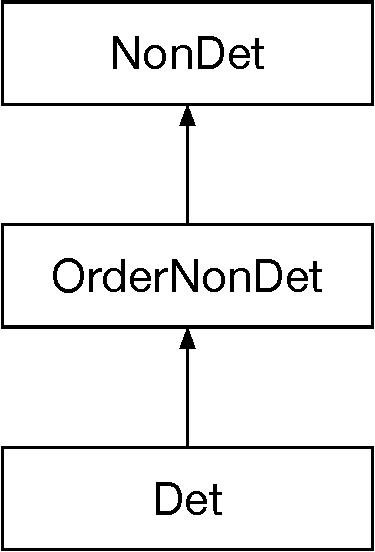
\includegraphics[scale=0.37]{detHierarchy}
%    \end{center}
%    \caption{Determinism type qualifier hierarchy}
%    \label{fig:determinism-hierarchy}
%\end{figure}

We defined a type system
that allows programmers to express (non)determinism properties.
The most novel part of our analysis is how it handles collections that will
contain the same values, but
possibly in a different order, on different runs.


%\todo{This is the first mention of
%    the determinism type system, and the first mention of types since the
%    abstract.  This is sudden and unexpected, and it will confuse readers.
%    You need to say that you will take this approach to solving the problem!}
%\todo{The introduction of the type
%    qualifiers is too sudden, too.  What are type qualifiers?  How are they
%    used?  Why does a reader care?  You should say that every expression in
%    the program is classified as one of the following categories.}

A type abstracts or restricts the set of possible
run-time values that an expression may evaluate to and the operations that
may be performed on it.
A programming language provides \emph{basetypes}, such as \<Int>.
A \textit{type qualifier} on a basetype adds additional constraints;
that is, it reduces the size of the set of values.
An example type qualifier is \<Positive>, and a type (which combines a qualifier
and a basetype) is \<Positive Int>.

The core of the determinism type system
is the following type qualifiers:
\begin{itemize}
    \item \<NonDet> indicates
    that the expression might have different values in two different executions.
    \item \<OrderNonDet> indicates that the expression is a collection or
    a map that contains the same elements in every execution, but possibly
    in a different order.
    \item \<Det> indicates that the expression evaluates to equal values in
    all executions; for a collection, iteration
    also yields the values in the same order.
\end{itemize}
% Every expression in a program is classified as either \<NonDet>, \<OrderNonDet>, or \<Det>.
%\todo{In a \LaTeX\ paper, use the standard mathematical symbols, not ASCII
%  approximations to them.}
The subtyping relationship among the type qualifiers is \<Det> $\sqsubseteq$ \<OrderNonDet> $\sqsubseteq$ \<NonDet>.
%\Cref{fig:determinism-hierarchy} shows the subtyping
%relationship among the qualifiers.
% Programmers can write these type qualifiers to specify their program's behavior. 
The following code is an example of a valid program that type checks. 
%\todo{This code is in poor style.  It assigns to a formal parameter, which
%  is unusual, it performs computation that is ignored (because its return
%  type is void).  Always make your examples as realistic as possible.  One
%  reason is that the code will be easier to read and less surprising or
%  distracting to readers.  Another reason is that if your code is
%  unrealistic, then readers will get the impression that your system is
%  impractical (because you couldn't think of a single real-world
%  application).  Make this code more realistic, or even use an example from
%  one of the libraries or programs.}
\begin{Verbatim}
public class Accesses {
    public NonDet int field1;
    public NonDet int field2;
        void setFields(NonDet int arg1, 
        Det int arg2) {
            field1 = arg1;
            field2 = arg2;
    }
}
\end{Verbatim}
%\todo{The use of ``type'' is confusing.  The paper improperly uses it for
%  qualifiers and return values.  Use the proper term.  When talking about a
%  type, use a type as you just defined it, not just a qualifier.}
All the assignments in this program 
satisfy the subtyping relationships.
 
The following method (From Junit~\cite{junit}), however, doesn't type check.
\begin{Verbatim}
public static Det Method Det[] getDeclaredMethods(
Class<?> clazz) {
    // Error: assignment type incompatible
    Det Method Det[] methods = 
    clazz.getDeclaredMethods();
    ...
    // Error: return type incompatible
    return methods;
}
\end{Verbatim}
The declared return type is annotated as \codeid{Det Method Det[]} (i.e a \<Det> array of \<Det Method> elements).
The call to \<getDeclaredMethods()> returns an array of type \codeid{Det Method OrderNonDet[]}
causing \theDeterminismChecker to issue a warning.
Note that \<getDeclaredMethods()> is a method in the JDK that provides no guarantees on the order of
the elements in the array that it returns and therefore we annotated its return type
to be an \<OrderNonDet> array.
%\todo{``The return type is not a subtype of the return type'' does not make
%  sense.  The first one is the type of the return value.  The second one is
%  the declared return type.  Also, as defined by the paper, \<Det> is not a
%  type.  The type should be \<Det int>.  Be careful about violating your
%  own definitions.}

%\todo{Cut the following sentence, which uses jargon like ``basetype'' that
%  has not been defined, and therefore is offputting and confusing to readers.}
%The basetypes of their elements can be specified independently of the collection basetypes.
%\todo{For the following sentence, show an example, or give the typing rule,
%  or both.}
An element type qualifier must be a subtype of the collection type qualifier.
For instance, the type \codeid{OrderNonDet Set<Det String>} is valid since the type qualifier
\<Det> is a subtype of the type qualifier \<OrderNonDet>.
%\todo{``subqualifier''?}  
The type \codeid{OrderNonDet Set<NonDet String>} is invalid because the element type qualifier (\<NonDet>) is not a subtype of the collection type qualifier (\<OrderNonDet>)
%\todo{Same
%    comment about types.}.
%\todo{\<NonDet> is not a type, so it cannot be the element
%  type.} 

%\OurTypeSystem checks all the standard typing rules\todo{``all the standard
%  typing rules'' is too glib.  It denigrates the reader by implying that
%  the reader ought to know this already, or that the paper is intended only
%  for a narrow audience with a specific technical background.  Make the
%  paper more welcoming.  Give a couple examples, and maybe even show source
%  code for them.}
%of an object-oriented programming language where the types have these
%additional type qualifiers.
%\todo{The following three things are the same.  Why are they listed as
%  different?  Also, their purpose is to reduce false positive warnings,
%  rather than to enable better reporting of true positives.  Also, try to
%  explain terms when you introduce them.  If you don't have space for that,
%  then ask yourself if this point is important enough to include in the paper.}

\subsubsection{Behavior of order-nondeterministic collections}\label{sec:ond-behavior}
A collection with the type qualifier \<OrderNonDet> has special properties. We elaborate on these 
properties with examples below:
%\todo{Like other parts of the document (and as noted by the referees), this
%  feels vague.  Make it more concrete, with examples or with specific explanation.}

\begin{enumerate}
    \item
    The individual elements retrieved from it have the type qualifier \<NonDet>.  This
    affects access, iteration, searching, etc.
%\todo{
%    The font size is different here than earlier in the paper.  Be
%  consistent.  
%  Also, the comment is inconsistent with the code, which lacks
%  the qualifier.  The comment is irrelevant because you can just correct
%  the code.  The paper is assuming that all qualifiers are explicit.  Do
%  the same in the next two examples.}
    \begin{Verbatim}
OrderNonDet HashSet<Det String> set; 
NonDet String elem = set.iterator().next();
    \end{Verbatim}
    \item
    Size-related operations return a deterministic result.  This affects
    queries of whether an iterator has more elements.
    \begin{Verbatim}
OrderNonDet HashSet<Det String> set; 
Det String elem = set.size();
    \end{Verbatim}
    \item
    If the collection is sorted, or its elements are placed in a collection
    that does sorting, the result is deterministic.
    \begin{Verbatim}
OrderNonDet ArrayList<Det String> lst;
Det ArrayList<Det String> sortedList = 
lst.sort();
    \end{Verbatim}
\end{enumerate}

%%  LocalWords:  NonDet OrderNonDet Det basetype offputting basetypes
% LocalWords:  subqualifier

\section{Evaluation\label{sec:results}}
To evaluate the usability of \theDeterminismChecker,
we applied it to the Randoop test
generator~\cite{PachecoLEB2007}.
Randoop is intended to be deterministic, when invoked on a deterministic
program~\cite{randoop-manual}.\footnote{Users of Randoop can pass in a different seed in order to
    obtain a different deterministic output.  Randoop has command-line
    options that enable concurrency and timeouts, both of which can lead to
    nondeterministic behavior.}
However, Randoop was not deterministic.  This caused the developers
problems in 
reproducing bugs reported by users, 
reproducing test failures during development, and
understanding the effect of changes to Randoop by comparing executions of two
similar variants of Randoop.

We first wrote specifications for libraries Randoop uses, such as the JDK,
JUnit, and plume-util.
Then, we wrote type qualifiers in the Randoop source code to express its
determinism specification.
Finally, we ran
\theDeterminismChecker.  Each warning indicated a mismatch between the
specification and the implementation.  We addressed each warning by changing our
specification, reporting a bug in Randoop, or suppressing a false positive warning.

\TheDeterminismChecker found \numRandoopBugs previously-unknown nondeterminism bugs in Randoop.
The Randoop developers accepted our bug reports and committed fixes to the repository. An example
of a severe bug follows, according to the Randoop developers' categorization:

\begin{itemize}
    \item
    \textbf{HashSet bug}: Suppose that in the code under test, a type variable's lower or upper
    bound has a type parameter that the type variable itself does not have. Then Randoop is nondeterministic.
    This situation does occur, even in Randoop's test suite.
    The developers fixed this by changing a \<HashSet> to \<LinkedHashSet>
    (commit c975a9f7, shown in \cref{fig:randoop-bug-hashset}).
    \TheDeterminismChecker confirmed that 
    25 other uses of \<new HashSet> were acceptable, as were 15 uses of \<new HashMap>.
\end{itemize}

\section{Research Contributions\label{sec:contributions}}
This paper makes the following contributions:
\begin{enumerate}
  \item We designed a type system for expressing determinism properties.

  \item We implemented the analysis, as a pluggable type system for Java, in a
    tool called \theDeterminismChecker.

  \item In a case study, we ran our analysis on a 24 KLOC project that
    developers had already spent weeks of testing and inspection effort to
    make deterministic.  \TheDeterminismChecker
    discovered 5 instances of nondeterminism that the developers had
    overlooked.
\end{enumerate}



\bibliographystyle{IEEEtran}
\bibliography{paper,bibstring-unabbrev,ernst,testing,types,crossrefs}

\end{document}
